\subsection{Leuchtmittel}
\subsubsection{Prinzipien}
Arbeiten Sie folgende Aufgabenstellung durch:

\question{Nach welchen Prinzipien funktioniert die Umwandlung elektrischer Energie in Licht?}
Nach den Prizipien der Temperaturstrahler, Gasentladungslampen und LEDs.

\subsubsection{Beleuchtungskörper}

Arbeiten Sie die unten aufgelistete Aufgabenstellung durch.

\clearpage

\begin{enumerate}
    \item   \question{Skizzieren und erklären Sie die induktive Schaltung einer Leuchtstofflampe mit konventionellem Vorschaltgerät}\\

            \begin{figure}[!htp]
                \centering
                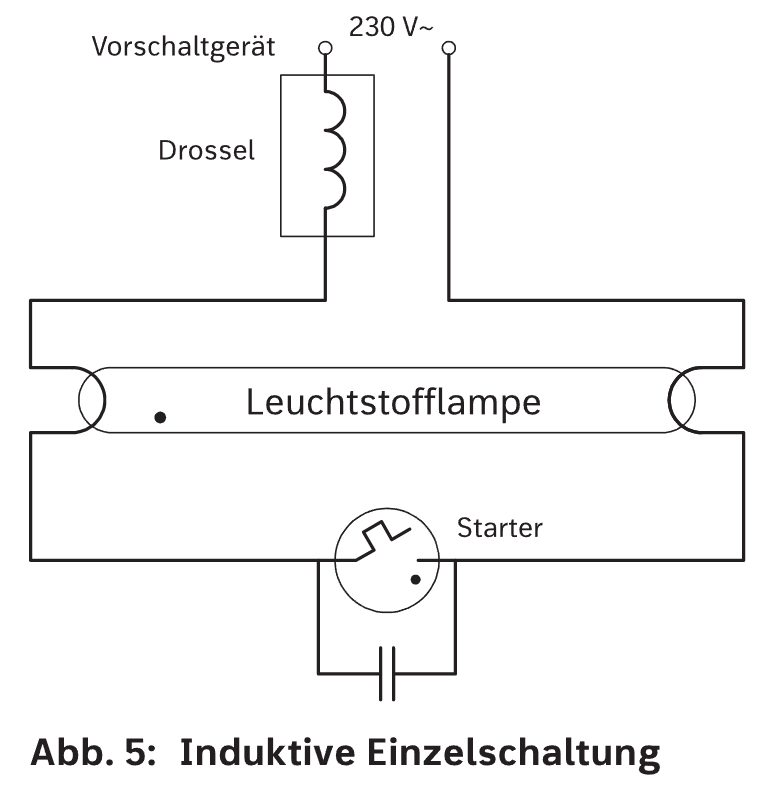
\includegraphics[scale = 0.3]{img/induktive_einzelschaltung.png}
            \end{figure}

    \item   \question{Skizzieren und erklären Sie die kapazitive Schaltung einer Leuchtstofflampe mit konventionellem Vorschaltgerät. Wo wird diese Schaltung eingesetzt, welche Vorteile hat sie?}\\
            \begin{figure}[!htp]
                \centering
                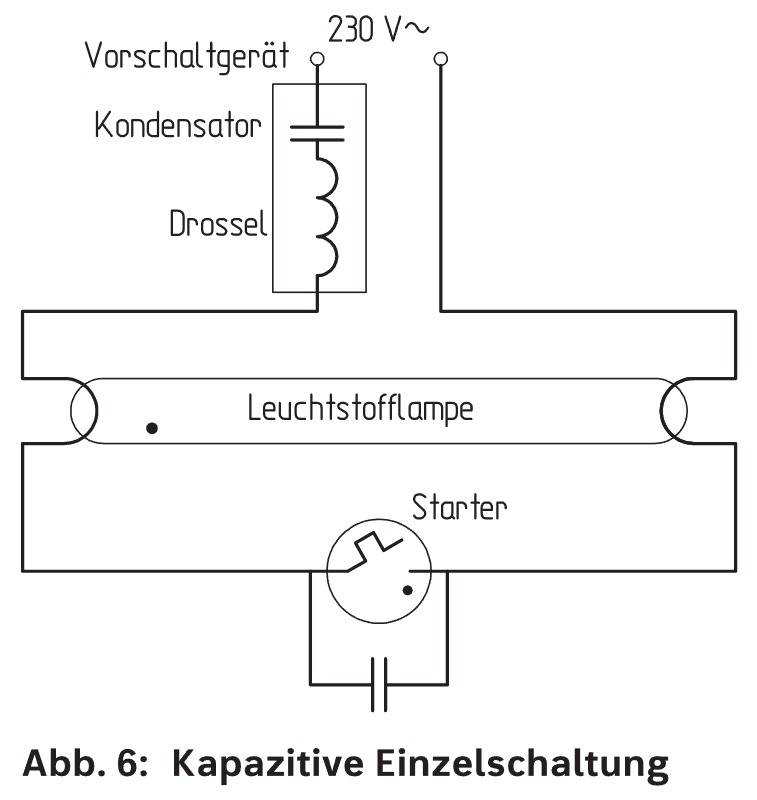
\includegraphics[scale = 0.3]{img/kapazitive_einzelschaltung.png}
            \end{figure}

            \begin{itemize}
                \item Kompensation der induktiven Last (Anstreben $\cos\left(\varphi\right) = 1$)
            \end{itemize}

            \clearpage
    
    \item   \question{Skizzieren und erklären Sie die Duo-Schaltung bei Leuchtstofflampen mit konventionellen Vorschaltgeräten. Wo wird diese Schaltung eingesetzt, welche Vorteile hat sie?}\\
            
            \begin{itemize}
                \item Kompensation der induktiven Last (Anstreben $\cos\left(\varphi\right) = 1$)
                \item Reduktion von Flackern durch zeitlich verschobenen Nulldurchgang zwischen z.B. zwei Tuben
            \end{itemize}

            Nutzung bei großflächige Anwendungen.

            \begin{figure}[!htp]
                \centering
                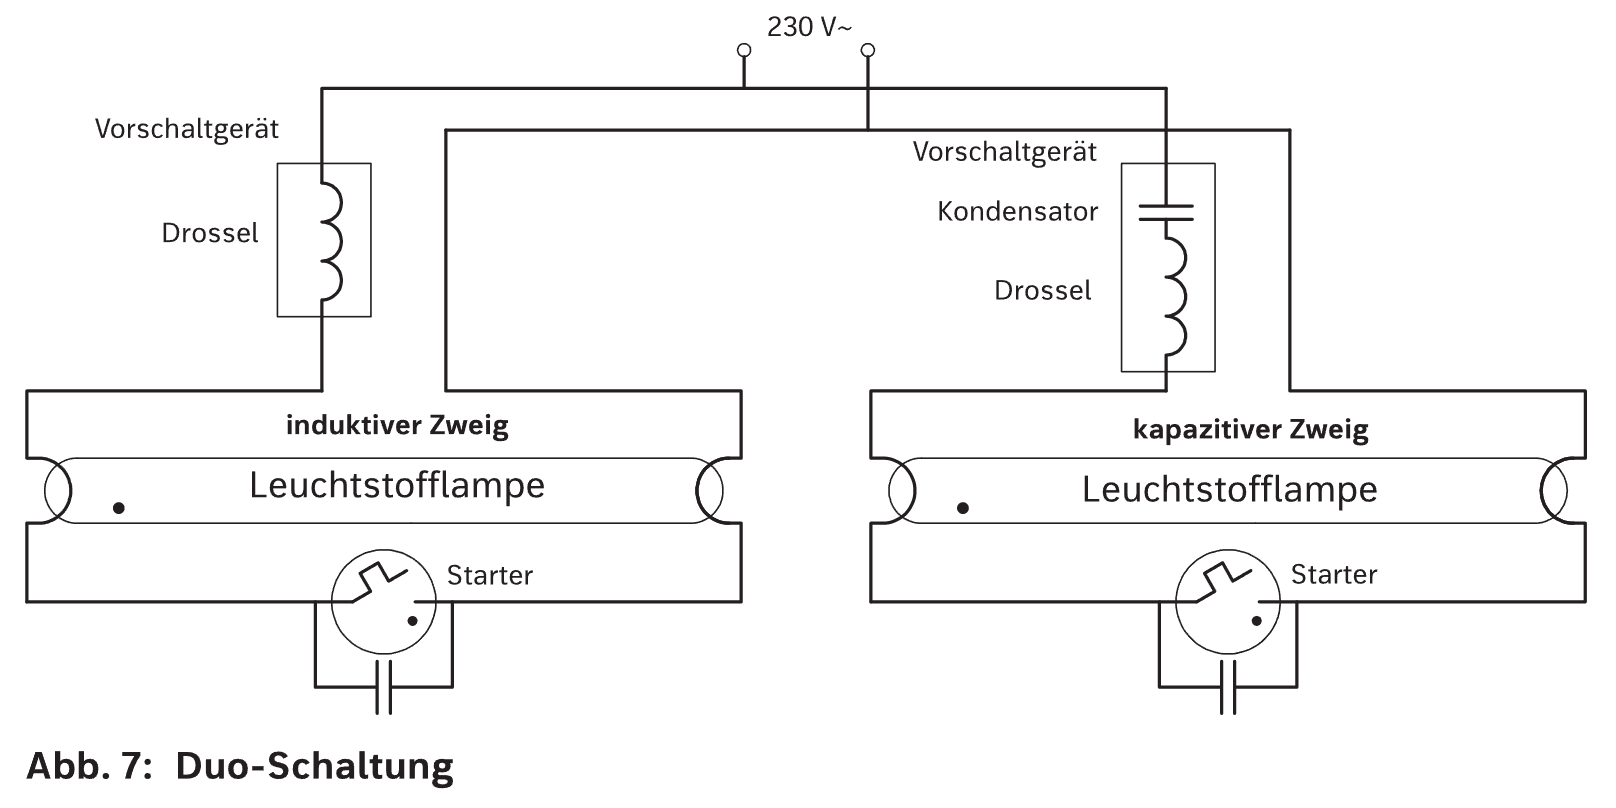
\includegraphics[scale = 0.3]{img/duo_schaltung.png}
            \end{figure}

    \item   \question{Wie wird bei Leuchtstofflampen der Zündvorgang hervorgerufen? Welche Vorschaltgeräte werden unterschieden und welche Vor- und Nachteile haben diese Vorschaltgeräte?}\\
    
    Mit Hilfe des Startes wird der Zündvorgang eingeleitet. Prinzip von einem Starter:
    \\1.    Lampe einschalten: Volle Spannung am Starter - Bildung einer Glimmentladung in der Edelgasatmosphäre - Erwärmung der Bimetallstreifen
    \\2.    Kurzschließen der Glimmstrecke durch die starke Biegung der Bimetallstreifen - Aufheizung der Lampenelektroden
    \\3.    Glimmentladung stoppt, Bimetallstreifen kühlt ab und öffnet - Unterbrechen von Heizkreis
    \\4.    An der Drosselspule tritt eine Selbstinduktionsspannung auf und dadurch erfolgt die Zündung

    \item   \question{Nach welchem Prinzip funktioniert eine Leuchtstofflampe?}\\
            Durch Gasentladung und Fluoreszenz.

            \clearpage
            
    \item   \question{Welche Gasentladungslampen kennen Sie und wo werden diese angewendet?}\\
    
            \begin{itemize}
                \item Natriumdampfhochdrucklampen\\
                    Beleuchtung von Straßen u. Plätzen. \\
                    In Neuanlagen werden statt Niederdrucklampen fast ausschließlich Hochdrucklampen verwendet.

                \item Natriumdampfniederdrucklampen\\
                    Ausfallsstraßen, Hafenanlagen, Schiffswerfen, Lagerhallen, u.ä.\\
                    Werden verwendet wenn Preis im Vordergrund steht. Keine Farbwiedergabeeigenschaften werden benötigt.

                \item Xenonlampen\\
                    Nach Beispielen Fragen. Laut Wikipedia:\\
                    Fahrzeugscheinwerfer, Großkinofilmprojektoren, Leuchtürme, für Wissenschaftliche Anwendungen
            \end{itemize}

    \item   \question{Lichttechnik: Welche thermischen Strahler kennen Sie und welche Vor- und Nachteile haben diese?}\\
            
            \begin{itemize}
                \item Glühlampe\\
                    Vorteile: Kontinuierliches Spektrum, hohe Farbtreue
                    Nachteile: Schlechter Wirkungsgrad (Große Wärmeverluste). Sehr viele Frequenzanteile im IR.

                \item Halogenlampen (Vor- u. Nachteile siehe unten)
            \end{itemize}


    \item   \question{Nach welchem Prinzip funktioniert eine Halogenleuchte? Welche Vor- und Nachteile bietet eine Halogenleuchte gegenüber anderen Leuchtmitteln?}\\
    
    Um das abschlagen von Wolfram am Glaskolben zu verhindern, wird bei dieser Lampe Jod eingebracht. In Lampenkolbennähe bildet
    sich Wolframjodid, das in Wendelnähe durch die hohe Temperatur wieder in Wolfram und
    Jod zerfällt.
    
    Da Glaskolben und Wendel verschiedene Temperaturen besitzen, kommt es zu einem
    Kreisprozess, und das vom Leuchtkörper abgetragene Wolfram wird nach vorübergehender
    Bindung an Jod wieder in Wendelnähe zurückgebracht.
    
    Niederschlagen von Wolfram am Kolben wird verhindert.
    
    Wegen der höheren Temperatur wird Quarzglas verwendet.
    
    Halogenglühlampen haben die gleichen Betriebseigenschaften wie gasgefüllte Glühlampen.

            Fragen: Evntl. Mehr Nachteile?\\
            Vorteile: Kleine Abmessungen, hohe Lebensdauer, hohe Lichtausbeutung (bis zu $27\frac{\textnormal{lm}}{\textnormal{W}}$), kein Lichtstromabfall durch Kolbenschwärzung\\
            Nachteile: Schlechter Wirkungsgrad, Frequenzanteile liegen überwiegend im IR.
\end{enumerate}